\documentclass{article}
\usepackage{graphicx}
\usepackage[margin=1.5cm]{geometry}
\usepackage{amsmath}

\begin{document}

\title{Wednesday Reading Assessment: Unit 7, Power and Conservation of Energy}
\author{Prof. Jordan C. Hanson}

\maketitle

\section{Conservation of Energy}

\begin{enumerate}
\item A particle of mass m is hung from the ceiling by a massless string of length 1.0 m, as shown in Figure \ref{fig:pend}. The particle is released from rest, when the angle between the string and the downward vertical direction is 30 degrees.
\begin{figure}[ht]
\centering
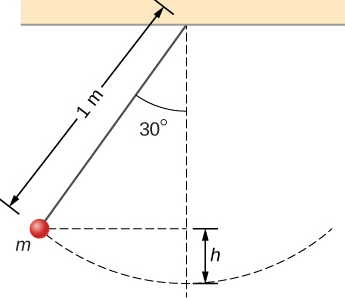
\includegraphics[width=0.4\textwidth]{pend.png}
\caption{\label{fig:pend} A particle hung from a string constitutes a simple pendulum. It is shown when released from rest, along with some distances used in analyzing the motion.}
\end{figure}
\item Show using trigonometry that the height of the pendulum is given by $h = L(1-\cos\theta)$. \\ \vspace{2cm}
\item What is the gravitational potential energy as a function of the angle $\theta$? \\ \vspace{2cm}
\item What is its speed when it reaches the lowest point of its arc, if the initial angle is 30 degrees?
\end{enumerate}
\end{document}